%% $Id: amr.tex,v 1.29 2007/04/22 13:50:54 benkirk Exp $
\chapter{An Adaptive Mesh Refinement Software Framework\label{chap:amr}}

%%%%%%%%%%%%%%%%%%%%%%%%%%%%%%%%%%%%%%%%%%%%%%%%%%%%%%%%%%%%%%%%%%%%%%%%%%%%%%%
  Adaptive Mesh Refinement (AMR) allows for efficient numerical simulation because the spatial mesh resolution is optimally adapted in some sense for a given problem.   This chapter will introduce key concepts and introduce data structures which are particularly well-suited for use in the AMR applications considered here.  Chapter~\ref{chap:parallel} will then address the implementation of adaptive methods on parallel computers.  Finally, Chapters~\ref{chap:bio} and~\ref{chap:compressible} will present application studies which apply the adaptive techniques discussed in this chapter.

The concepts discussed herein have been implemented concretely in the \libMesh{} open-source software library.  The library was initiated by the author to aid in (i) testing the ideas presented here  and (ii) to enable the application of parallel AMR solution schemes to a wide range  mathematical models for physical systems.  The library itself is not tied to any particular application, and consequently is being adopted by a number of researchers in the U.S. and abroad for use in a wide range of applications.

%%%%%%%%%%%%%%%%%%%%%%%%%%%%%%%%%%%%%%%%%%%%%%%%%%%%%%%%%%%%%%%%%%%%%%%%%%%%%%%
\section{Introduction}

A primary goal of AMR is to enable more efficient and reliable numerical simulations.  Some
examples for problems of boundary layer type and nonlinear problems
with singularities in~\cite{carey_bail_2004} demonstrate the
effectiveness of AMR in flow and transport simulations. In particular,
AMR can significantly increase the range of problems that can be
attempted given a limited set of resources on workstation-class (or larger) systems.  However, it is also obvious that adaptive
meshes imply a need for more general data structures. This, in turn,
leads to increased complexity, especially in parallel distributed
AMR simulations.

In a typical adaptive refinement scheme, the solution on a given mesh
is post-processed to obtain local error indicators that provide
feedback for selective local mesh
refinement~\cite{carey_gridbook,carey_bail_2004}. The basic approach
for the simulation of partial differential equations in parallel with AMR applied to a steady state problem proceeds
as follows:
\begin{enumerate}
\item{First, an initial mesh is generated, the mesh is partitioned to
  subdomain meshes, and a solution is computed in parallel on this
  parent mesh (stabilization may be required for flow or transport in
  which convective effects are significant at this mesh scale).  The
  details of the mesh partitioning scheme will be deferred until
  Chapter~\ref{chap:parallel}.}
  
\item{Next, a posteriori error indicators are computed from the
 approximate solution on the current mesh and a subset of cells are
 flagged by the error indicator.}

\item{These cells are subdivided and continuity constraints are
  enforced (in the subsequent solve step) at ``hanging'' nodes on
  element edges or faces shared with adjacent, unrefined elements.}

\item{If the load balance has not significantly changed as a result of
  the local refinement step, then repartitioning is not needed at this
  stage and the parallel solution over the existing partition continues
  with the new adapted mesh. Otherwise, repartitioning is carried out
  with due attention to the unbalanced tree data structure and the
  edge-neighbor information required on the partition interface as
  described below.}
\end{enumerate}

In solving evolution problems, the same general approach is applied
within each time step.  The solution and the adapted, partitioned mesh
at the end of the previous time step become the starting solution and
mesh for the next time step.  Simulation proceeds as in the static AMR
situation above except that now coarsening of previously refined cells
also becomes more important due to the changing spatial behavior of the
solution in time.

Note, in particular, that the steps outlined above are in general independent of \emph{what} is actually being simulated.  It is therefore possible to separate the software implementation which enables parallel simulations using adaptive mesh refinement from the physics-specific code required for a given application.  This approach was taken as part of the present work by developing the \libMesh{} library which in a sense amortizes the effort required to implement a parallel adaptive capability by allowing the supporting software infrastructure to be used for a wide range of problems.  A similar approach has been applied most notably by researchers at Sandia National Laboratories in the \texttt{SIERRA} framework which is used for massively parallel simulations of multiphysics applications~\cite{sierra}.

The remainder of this chapter discusses several key data structures which have been developed for use in the present work. An overview of object-oriented scientific computing software is first presented as this is the paradigm used to implement the relevant data structures. The discussion will focus on how these data structures can be used to perform adaptive mesh refinement simulations without regard to the particular computing paradigm used.  The subsequent chapter will then consider specific issues which arise when this approach is applied on parallel, distributed memory computers.

%%%%%%%%%%%%%%%%%%%%%%%%%%%%%%%%%%%%%%%%%%%%%%%%%%%%%%%%%%%%%%%%%%%%%%%%%%%%%%%
\section{Object-Oriented Scientific Computing\label{sec:amr_oop}}
In recent years the performance of the \cpp{} programming language has improved to the point that it provides a viable option for implementing high performance, object-oriented software.  A complete discussion of object-oriented ideas and the features of a given programming language is outside the scope of this work. However, a cursory overview of object-oriented approaches (and their contrast to procedural approaches) is worthwhile as it provides the necessary background for the data structures described later in this chapter.

Two distinct paradigms for implementing software algorithms are procedure-oriented approaches and object-oriented approaches.  The procedural approach has been the mainstay of scientific computing for decades, dating back to the earliest versions of the \texttt{FORTRAN} programming language.  In this approach basic computational kernels are constructed as a set of procedures which operate on some set of data.  Implicit in this approach is an assumption as to the specific data types used to implement a given algorithm.  One consequence of this is that the data storage and procedure implementation are intimately related.  For example, suppose a standard array were used to store the individual elements of a vector.  If for some reason it were decided that a linked-list would be a more efficient data structure, due to dynamic insertion and removal of elements for example, then substantial changes to all code which uses such a vector would be required.

By contrast, object-oriented approaches define specific \emph{classes} which present characteristics and defined behaviors.  An \emph{object} is simply an instance of a given class.  A significant benefit of objects is \emph{encapsulation}, which is the ability to separate actual data from operations which are performed on the data.  Returning to the vector example, in an object-oriented approach the specific data structure used to store numeric values could be completely encapsulated within an object, and code which uses such an object need not have any insight or access to this data structure. In this way encapsulation allows well-written objects to change algorithmic implementation or data storage techniques without affecting external code.   For this and many other reasons, object-oriented programming is generally considered to create more maintainable and extensible software.  Consequently, these approaches have become standard in many aspects of software engineering.  The adoption of object-oriented techniques in the field of scientific computing has proceeded at a slow pace but is certainly gaining momentum.  



%%%%%%%%%%%%%%%%%%%%%%%%%%%%%%%%%%%%%%%%%%%%%%%%%%%%%%%%%%%%%%%%%%%%%%%%%%%%%%%
\clearpage
\section{Data Structures for Adaptive Mesh Refinement Simulations\label{sec:amr_data_structures}}
Data structure selection is critically important for effective AMR
implementation~\cite{libMeshPaper,BHK07}. In the results presented
later, a tree structure is used.  In this data structure each element
can directly address both its ``parent'' and its ``children.'' No assumptions
are made here as to how many children an element may have.
\begin{figure}[hbtp]
  \begin{center}
    \subfigure[one level of refinement mismatch.\label{fig:amr_levels_a}]{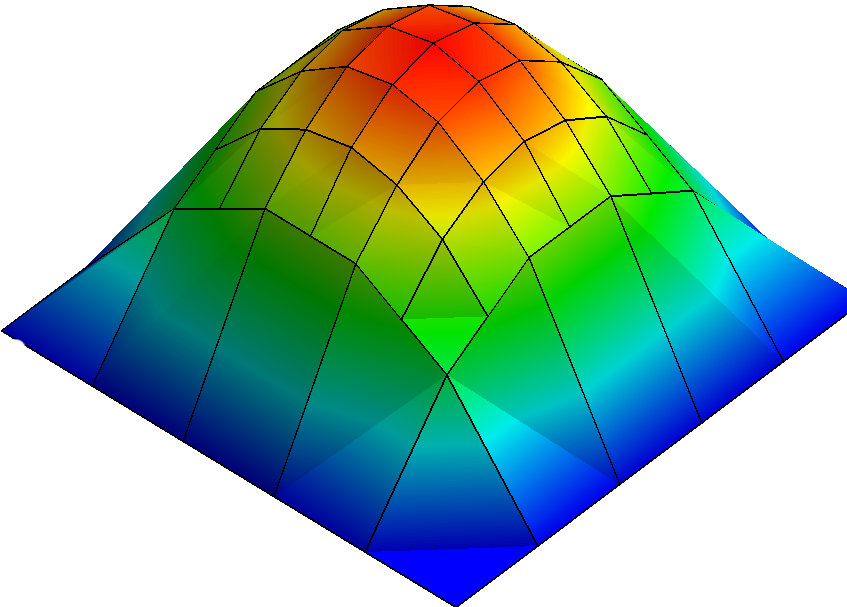
\includegraphics[width=.48\textwidth]{figures/amr_levels/01}}
    \subfigure[three level of refinement mismatch.\label{fig:amr_levels_b}]{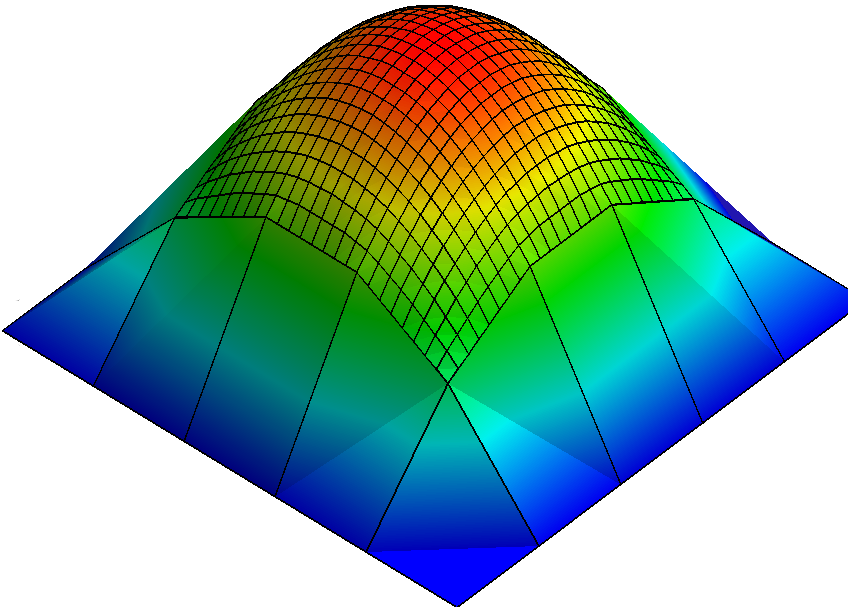
\includegraphics[width=.48\textwidth]{figures/amr_levels/03}}
    \caption{Solution to a Poisson problem on meshes with one and three levels of mismatch at element interfaces.\label{fig:amr_levels}}
  \end{center}
\end{figure}
Additionally, each element can access its face neighbors. This data
structure enables very flexible refinement strategies.  For example,
the familiar ``level-one'' restriction, in which adjacent elements are
allowed to differ by only one level of refinement as shown in
Figures~\ref{fig:amr_levels_a} and~\ref{fig:amr_data_structuresa}, is
not required by the present data structure.  A depiction of a mesh
which does not conform to the level-one rule is shown in
Figure~\ref{fig:amr_levels_b}.
\begin{figure}[htp]
  \centering
  \subfigure[Level-one refinement with a hanging node\label{fig:amr_data_structuresa}]{%
    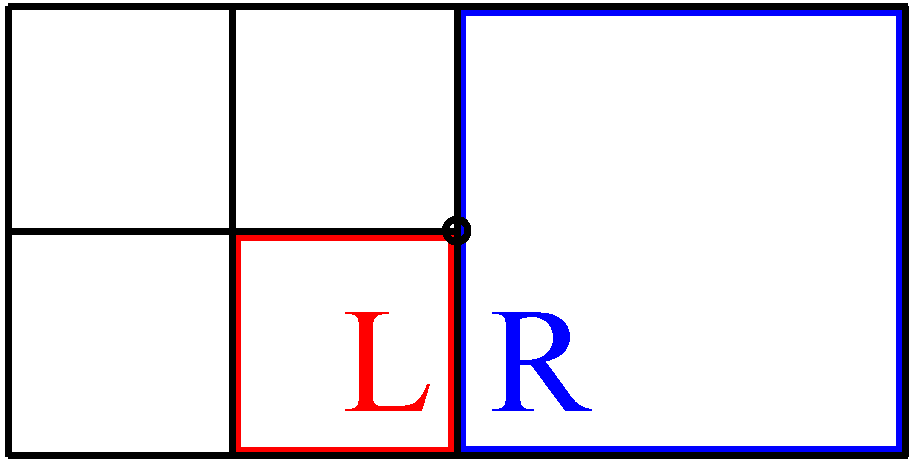
\includegraphics[height=.3\textwidth]{figures/dof_constraints/old_way}}
  \hspace{1em}
  \subfigure[Corresponding parent-child relationship\label{fig:amr_data_structuresb}]{%
    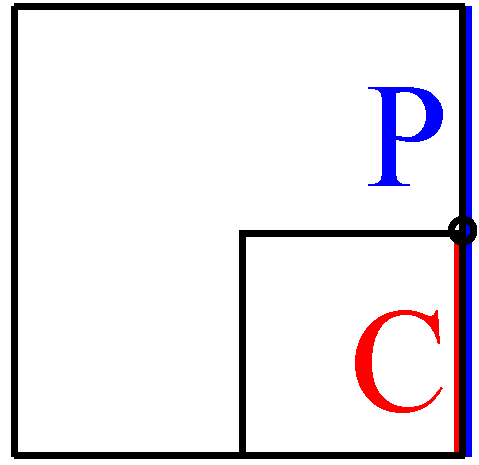
\includegraphics[height=.3\textwidth]{figures/dof_constraints/new_way}}
  \caption{AMR data structures: neighbor and parent-child relationships.}
  \label{fig:amr_data_structures}
\end{figure}

For continuous finite element approximation spaces, the finite element
basis obviously must be continuous throughout the domain.  Refinement
interfaces like those shown in Figure~\ref{fig:amr_levels} therefore
require special treatment to ensure this continuity.  The parent-child
relationship depicted in Figure~\ref{fig:amr_data_structuresb} is used
in the present work to generate the required inter-element continuity
constraints. This parent-child strategy is particularly useful on
distributed memory machines since only local data is required.  The
general approach used in this work is to constrain the child element
to be continuous with a parent element.  That is, on $\Omega_P \cap
\Omega_C$:
\begin{eqnarray}
  u_C &=& u_P \nonumber \\
  \sum \alpha_i \phi_i^C &=& \sum \beta_i \phi_i^P \nonumber \\
  \bv{A} \bv{\alpha} &=& \bv{B} \bv{\beta} \nonumber \\
  \bv{\alpha} &=& \bv{C} \bv{\beta} \nonumber
\end{eqnarray}

Furthermore, since no assumptions are made about neighboring elements,
this approach admits arbitrary refinement mismatch at element
interfaces. This case of arbitrary element mismatch can be
handled by introducing \emph{recursive constraints}: If $\bv{u}_a = \bv{C}_b \bv{u}_b$ and
$\bv{u}_b = \bv{C}_c \bv{u}_c$ then this implies $\bv{u}_a = \bv{C}_b \bv{C}_c \bv{u}_c$.
%\begin{wrapfigure}{R}{.4\textwidth}

This approach has been used in the \libMesh{} library to enable
adaptive mesh refinement simulations using a wide variety of finite
element types. Figure~\ref{fig:amr_hybrid} shows the solution to the
Poisson problem for an adapted hybrid mesh with mismatch in which the
constraints were treated using this method.
\begin{figure}[hbtp]
  \begin{center}
    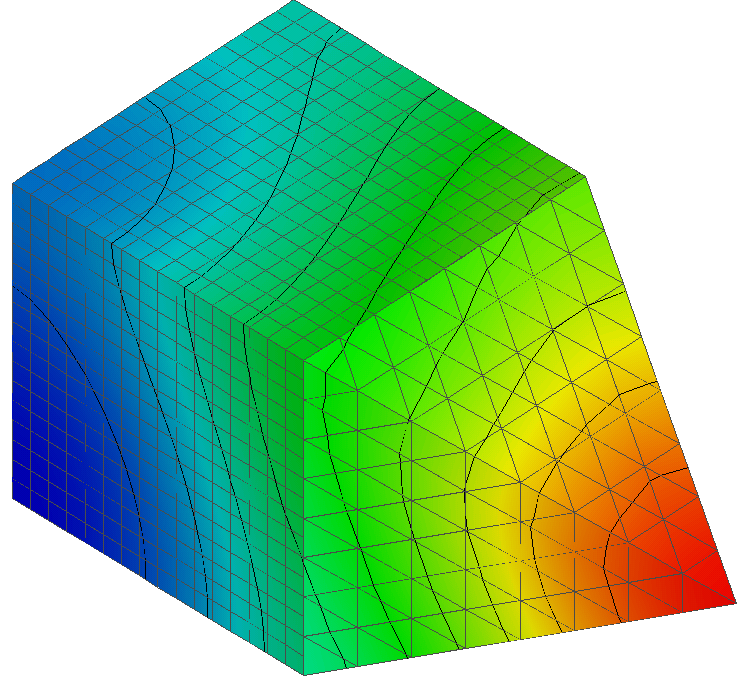
\includegraphics[width=.55\textwidth]{figures/amr_levels/pointy}
    \caption{Adaptive mesh refinement on a three-dimensional hybrid grid.~\label{fig:amr_hybrid}}
  \end{center}
%\end{wrapfigure}
\end{figure}
 The cube base region is meshed with triangular prisms, and the
pyramid region is composed of tetrahedra.  The approach has recently
been extended to the case of \emph{hp}-adaptive finite element
simulations in which the mesh is adapted spatially and the finite
element approximation space is modified to provide enhanced
convergence.

\subsection{Mesh}
The \texttt{Mesh} class is central to \libMesh{} and was one of the
first developed.  It provides a discrete description of a
$d$-dimensional object in $D$-dimensional space, where $(d,D)$ are 1,
2, or 3.  The class supports manifolds, so strictly speaking $d \le
D$.  The discretization is composed of elements and nodes which are
stored in the mesh, but the manner in which these data are stored is
encapsulated by abstract classes which present
implementation-independent interfaces to the user.  This data
encapsulation has allowed for re-factoring of the mesh class with
minimal impact on the external application programming interface.

A base class/derived class structure is used to implement mesh input/output in
various formats.  Virtual base classes describe the interface for mesh
input and output, and derived classes provide the actual I/O
functionality.  The library currently supports reading and writing a
number of unstructured mesh formats, including: the UCD format from
AVS, the I-deas UNV Universal format, Exodus~II from Sandia National
Labs, GMSH, TetGen, Tecplot (ASCII and binary), and the GMV format from Los
Alamos National Labs.  The initial mesh is assumed to be conforming
and provides the level-0 parent elements in the refinement hierarchy
described in Section~\ref{sec:elements_hierarchy}.

Custom iterator objects can be created to provide access to the
elements and nodes contained in a mesh.  The user can instantiate
iterators to access all the elements in the mesh or some meaningful
subset thereof.  The latter approach is useful, for example, during
parallel finite element matrix assembly on an adaptively refined mesh.
In this case, the user obtains iterators which traverse the set of
active elements (described in more detail in
Section~\ref{sec:elements_hierarchy}) which are owned by the local
processor.

The mesh class is designed to be extensible.  Encapsulating the stored
elements and nodes by providing access only through custom iterators
admits the possibility of providing different implementations for
specific classes of meshes.  The current \texttt{Mesh} implementation
assumes a fully unstructured, hybrid element mesh.  However,
algorithmic and storage-based optimizations for Cartesian grids,
block-structured grids, and grids with only a single type of element
could be added without changing the current interface.


\subsection{Degrees of Freedom\label{sec:dof_distribution}}
\enlargethispage{-\baselineskip}
The first finite elements implemented in \libMesh{} were the standard
Lagrange elements with nodal value degrees of freedom.  The library
has since been extended to a wider variety of finite element types.
Shape functions on more exotic finite elements can correspond to nodal
Hessian components, mid-edge normal fluxes, or orthogonal hierarchic
polynomials.  With many shape functions there may be no single
associated geometric
point.

The \texttt{DofObject} class handles these different types of 
degrees of freedom generically.  Examples of \texttt{DofObject}s
are element interiors, faces, edges, and vertices.  An element interior
has associated degrees of freedom for those shape functions whose
support is contained within the element.  Face degrees of
freedom correspond to shape functions contained within the two
elements sharing a face, edge degrees of freedom correspond to shape
functions for all elements sharing an edge, and vertex degrees of
freedom correspond to shape functions supported on all elements
sharing a single vertex.


\subsection{Nodes}
The \texttt{Node} class stores its $(x,y,z)$ location in space, as
well as additional state information including a unique \texttt{id} and its degree
of freedom indices.  The mesh data structure contains a complete list
of all nodes.  Nodes may be accessed directly by the user via
iterators, or indirectly through elements which are connected to the
nodes. Trivial operations which do not alter the mesh topology such as scaling, translating, or rotating a
mesh are performed directly on the nodes.

During the refinement process new nodes may be added to the mesh.
When two adjacent elements are refined, common nodes will exist on the
inter-element interface. This situation must be properly resolved to
achieve a valid discretization (i.e.\ with no duplicate nodes and
associated ``tears'' in the mesh).  A new node is created as a
weighted combination of existing nodes.  For each new node, a hash key
is constructed based on these weights and global \texttt{id}s of its
parent nodes.  If this key already exists in the map of new node keys,
the new node \emph{may} be a duplicate and is therefore compared to
any nodes with the duplicate key. (Note that if a ``perfect hash'' key
were devised this comparison would be unnecessary.)  Clearly, if the
new node is a duplicate it is then rejected. This procedure relies on
the near-uniqueness of the hash key and has been found to efficiently
resolves nodal connectivity for refined elements.

Similarly, coarsening the mesh can create ``orphan nodes,'' or nodes
that are no longer connected to any elements.  In an initial
implementation these orphan nodes were kept in place, so that they
could be re-connected to future elements that may appear in the
refinement process.  In particular, in transient applications with
some periodic behavior, elements will be created and destroyed
repeatedly, and it was thought that leaving the nodes in place could
speed up subsequent refinements.  However, numerical experiments
indicated that this approach did not provide an appreciable speedup,
and the default behavior is now to remove such orphan nodes.  After a
refinement/coarsening step the library simply counts the number of
elements connected to each node and removes those nodes with no
element connections.


\subsection{Elements}
\libMesh{} defines the abstract base class \texttt{Elem} which
defines the interface for a geometric element.  Concrete
subclasses of \texttt{Elem}, such as \texttt{Quad4} and
\texttt{Tet10}, are specialized via virtual function calls to return, for example, the correct number of nodes and sides when \texttt{n\_nodes()} and
\texttt{n\_sides()} are called on an \texttt{Elem} pointer.  The
complete list of geometric element types provided in \libMesh{} is shown in
Figure~\ref{fig:elem_class}.
\begin{figure}
  \begin{center}
    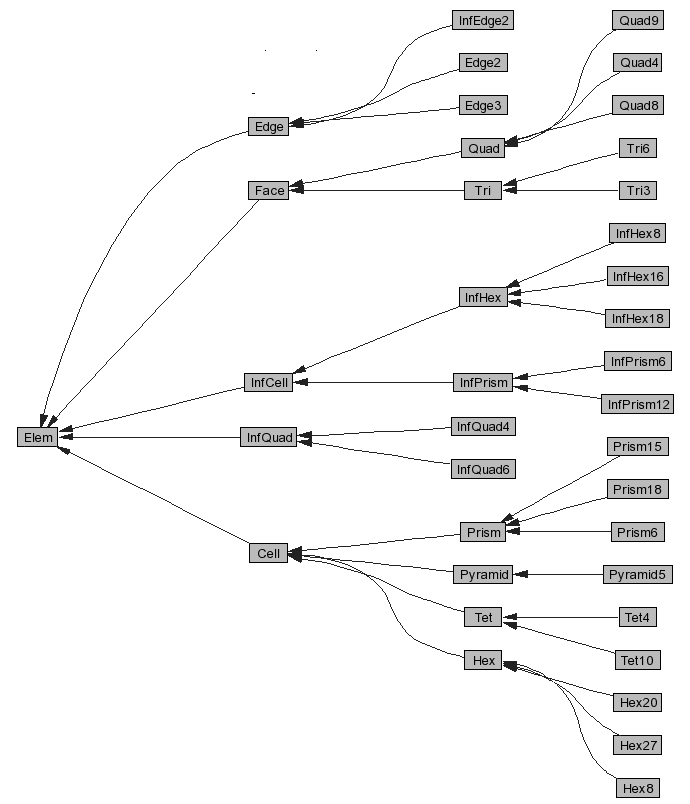
\includegraphics[width=.95\textwidth]{figures/data_structures/inherit_graph}    
    \caption{The \texttt{Elem} class hierarchy\label{fig:elem_class}}
  \end{center}
\end{figure}
Note that an \texttt{Edge} \emph{is} an \texttt{Elem} (in the polymorphic
sense) in 1D, and similarly for \texttt{Face} in 2D and \texttt{Cell} in 3D.
Implementations of all the standard geometric element types used in finite
element analysis including quadrilaterals, triangles, hexahedra, tetrahedra,
prisms, and pyramids, as well as a collection of infinite elements, are
provided in \libMesh.

\subsubsection{Nodal Connectivity\label{sec:elements_connectivity}}
Elements contain state information similar to nodes.  Elements store a
unique \texttt{id}, their processor \texttt{id}, and degree of freedom information.
Additionally, the element connectivity is stored as pointers to nodes.
This is a slight departure from the classic finite element data
structure, in which the element connectivity is defined in terms of
the nodal indices~\cite{becker_carey_oden_volume_1}.  On 32-bit
machines pointers and integers are both 4~bytes, so this choice does
not impose additional storage.  On 64-bit machines, however, pointers
are 8~bytes, which essentially doubles the amount of memory required
to store element connectivity.

This approach for storing the element connectivity was chosen so that
elements could have increased functionality in the absence of a
\texttt{Mesh} object.  A traditional connectivity scheme would require
the mesh to access the nodal locations of a given element.  This is
important, for example, when computing the map from a physical to
reference element or determining if a point lies inside an element.
By storing pointers to the nodes, the element can determine its
geometric connectivity directly.  This simplifies many functions in
the code by requiring the user to pass only an element instead of both
an element and the nodal locations. Additionally, this approach
reduces the amount of indirect memory addressing required for an
element to obtain nodal information as it may determine the physical
location of its nodes with a single pointer dereference.

\subsubsection{Face Neighbors\label{sec:elements_neighbors}}
Elements also store pointers to their face neighbors.  Two elements
are said to be face neighbors if they share a ``side,'' where a
``side'' is a node in 1D, an edge in 2D, and a face in 3D.  If an
element side is on the physical boundary of the domain there will be
no neighbor.  This is indicated in the code by a \texttt{NULL}
pointer, so locating the elements coincident with the boundary is
equivalent to finding all the elements with a \texttt{NULL} neighbor.
This is useful, for example, when applying boundary conditions.

After reading a mesh from disk, or performing mesh refinement, it is
necessary to construct the face neighbor information efficiently.  The
library handles this by looping over all the elements and then over
the sides of the element.  If a neighboring element has not been
located already the side of the element is constructed and a hash key
is computed based on the global indices of its nodes.  A map is then
queried to find any elements with sides matching this key, and they
are checked for a possible match. The neighboring element will have
the same side connectivity.  When the matching neighbor is located it
is removed from the map, therefore reducing the overall size of the
map.

The loop through the $N$ elements is $\mathcal{O}(N)$, while for a map
of size $M$ the lookup is $\mathcal{O}(\log M)$, so the resulting
algorithm has $\mathcal{O}(N\log M)$ complexity. In the current
implementation $M \le N$, yielding a worst-case
$\mathcal{O}(N\log N)$ algorithm.  Alternate approaches are possible
for which $M \ll N$ which could improve performance for very large
meshes.  For example, ordering the elements with a space-filling curve
before performing the neighbor search will ensure adjacent elements
are quickly located, reducing the maximum size of the map so that $M \ll N$.

Since constructing the side of an element is a common task, a special
proxy class called \texttt{Side} has been developed for this purpose.
This class essentially defines the side of an element as a new element
living in a lower spatial dimension and provides the connectivity
through a mapping from the original element.  This approach allows the
side of an element to be constructed rapidly, as the allocation and
population of a new connectivity array is not required.

\subsubsection{Element Refinement Hierarchy\label{sec:elements_hierarchy}}
Elements are refined upon user request via the ``natural refinement''
scheme.  In this approach $d$-dimensional elements are generally
refined into $2^d$ subelements of the same type. (Pyramid refinement
is an exception to this rule: refining a pyramid results in a
collection of pyramids and tetrahedral elements.)  Hanging nodes are
allowed at element interfaces and hanging degrees of freedom are
constrained algebraically using the technique discussed
previously. This approach was chosen because it is applicable for
general hybrid meshes with arbitrary types of elements, and in general
results in refined elements of the same type.  This latter point
ensures that refining an all-quad mesh in 2D produces an all-quad
mesh, for example.  Additionally, this approach results in refined
elements which are geometrically similar to the parent, thereby
preserving the initial element quality.

This refinement approach naturally yields a tree-like data structure.
Figure~\ref{fig:hierarchy} shows the quad tree-data structure which
results from refining a single quadrilateral element.
\begin{figure}[hbtp]
  \begin{center}
    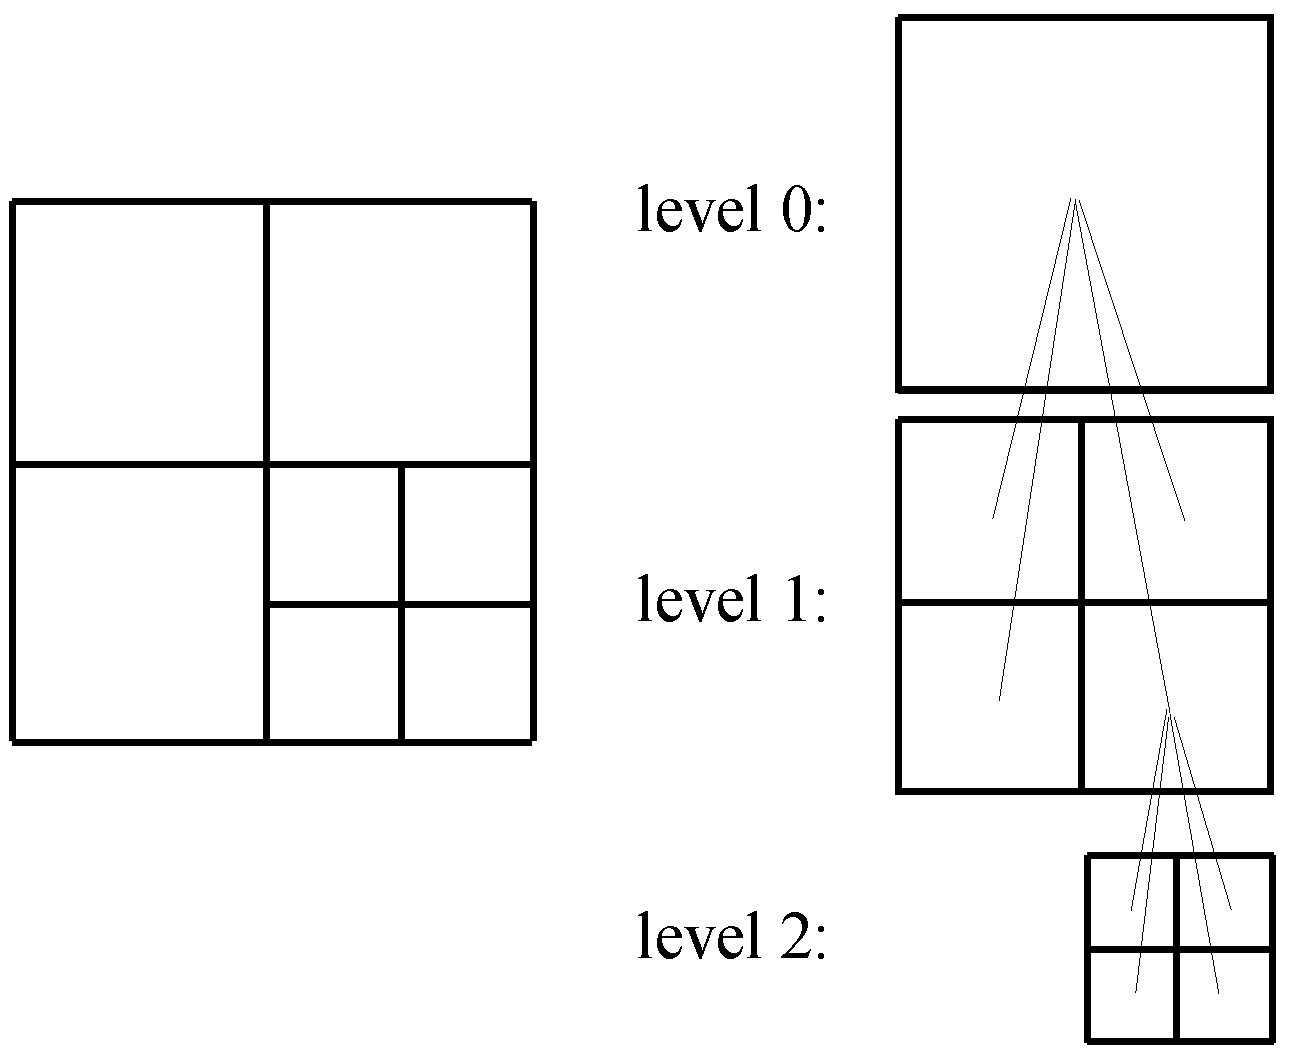
\includegraphics[width=0.7\textwidth]{figures/data_structures/hierarchy}
    \caption{Element refinement hierarchy for a 2D quadrilateral mesh.\label{fig:hierarchy}}
  \end{center}
\end{figure}
Each element has a pointer to its ``parent,'' and an array of pointers
to its ``children.''  The initial, level-0 elements are unique in that
they have no parent.  This is indicated in the code with a
\texttt{NULL} parent pointer.  Similarly, the active elements which
are used in finite element computations have no children, hence they
have a \texttt{NULL} array of children.  The level of a given element
may be determined recursively from its parent.  The user is allowed to
access any subset of the elements via iterators as discussed
previously.  The active ``leaf'' elements are commonly used in matrix
assembly, but intermediate levels could also be used in a multigrid
cycle, for example.

The element hierarchy is additionally used to locate hanging nodes in
the mesh which must be constrained.  As mentioned previously, elements
store pointers to neighboring elements which share sides.  These
neighboring elements are necessarily at the same level of refinement.
If an active element neighbors a refined element (also referred to as
an ``inactive'' element) then any degrees of freedom located on the
common side must be constrained.

The refinement hierarchy also naturally supports element
coarsening. In the case that all of the children of an element are
flagged for coarsening, the parent element simply deletes its
children, \texttt{NULL}s its children array, and becomes active again.
(Note that the neighbor connectivity of the parent is unchanged in
this process and therefore does not need to be regenerated.)  In
Figure~\ref{fig:hierarchy}, this would correspond to all the level-2
elements being deleted.  The resulting mesh would contain just the
active level-1 elements and their parent.  A consequence of this
approach to element coarsening is that the mesh cannot be coarsened
below the initial, level-0 mesh.  In many cases it is desirable to use
the coarsest level-0 mesh possible and allow the refinement process to
add elements only where they are needed.

Finally, the refinement tree can be exploited when enumerating
boundary conditions.  A data structure is provided which maps an
element and its relevant side(s) to a boundary condition
enumeration. (Note that, in keeping with the physics-independent
nature of the library, imposing the boundary conditions is left to the
user.)  By nesting the children such that boundary ``sides'' are
coincident with the same sides as the parent, this data structure can
be static and reused regardless of mesh level. This is implemented by
recursively returning the parent's boundary condition information for
the relevant side until the top-level parent is located and the map is
ultimately queried.

\textbf{Remark:} The element concept discussed here corresponds to the
geometric entities use in a discretization.  This is a distinct notion
within the library from the finite element approximation space used in
the numerical simulation.  This distinction allows for a convenient
separation of the geometric modeling function of \emph{elements} and
the approximation properties of associated \emph{finite elements}.
For example, a two-dimensional simulation using piecewise linear
Lagrange basis functions may use triangular and quadrilateral
elements, but the underlying finite element type is specified by the
use of a first-order Lagrange basis.

\subsection{Systems}
The abstract \texttt{System} class in \libMesh{} corresponds to a set
of one or more partial differential equations which are to be solved
on a given mesh.  \libMesh{} provides several concrete system
implementations including explicit, implicit, steady, transient,
linear, and nonlinear systems.  A system stores the solution values
for the degrees of freedom in a simulation, which may be either real
or complex valued.  Additionally, a system may contain additional
information (such as a sparse matrix) required for a particular
solution strategy.  In the current implementation a system is uniquely
tied to a given mesh, so a simulation that uses multiple meshes must
also solve multiple systems.

The \texttt{System} class provides a generic, customizable interface
which allows the user to specify the physics-dependent parts of an
application.  For example, in the case of an implicit system, users can
provide a function for matrix assembly or can derive their own class
and overload the matrix assembly operator.  Similarly, for transient
systems, the user may either provide an initialization function or
overload the initialization operator provided in the library.

Multiple systems may be tied to a given mesh to allow for loose
coupling of different physics.  This feature has been applied to
iteratively decouple the incompressible fluid flow and heat transfer
equations.  In this example two implicit systems are solved in an
iterative fashion.  Similarly, incompressible flows using pressure
projection operator splitting techniques have been solved using a
combination of loosely coupled explicit and implicit systems.

The library makes extensive use of \cpp{} templates to allow
complex systems to be constructed from simpler subsystems.  For
example, transient nonlinear systems are supported by combining a
transient outer loop with a nonlinear inner loop.  Templates are
useful in this setting because they allow simple components to be
combined into a complex algorithm. This leads to code reuse and
minimizes debugging efforts.


%%%%%%%%%%%%%%%%%%%%%%%%%%%%%%%%%%%%%%%%%%%%%%%%%%%%%%%%%%%%%%%%%%%%%%%%%%%%%%
\section{Finite Element Type Independence in Adaptivity\label{sec:element_independent_amr}}

A primary goal of \libMesh{} is extensibility: it should be easy for
experienced users to add new finite element types to the system with
minimal effort.  To make this possible, \libMesh{} includes
implementations for hanging node constraints,
solution restrictions to coarsened meshes, and solution projections to
refined meshes which are independent of the underlying finite element space.  When adding a new finite element to the library, developers
can first use these default implementations, only replacing them with
optimized element-specific implementations if necessary for
efficiency.

%\subsection{Hanging Node Constraints}
When using the hierarchical mesh refinement capabilities provided by
\libMesh, the resulting meshes are non-conforming, with ``hanging
nodes'' on sides where coarse elements and more refined elements meet.
The approach described previously for generating these constraints is generally applicable to arbitrary element types.

%% On these sides, the spaces of function values and fluxes on the coarse
%% element are strict subspaces of the values and fluxes which are
%% possible on the refined neighbors.  Ensuring $C^r$ continuity
%% between these sp\-aces requires constraining some or all of
%% the refined element degrees of freedom.

%% Degrees of freedom on the side of a fine element must be expressed in
%% terms of degrees of freedom on the overlapping side of a neighboring coarse
%% element.  The goal is to ensure that all function values and
%% derivatives up to the required continuity level are equal.  We 
%% impose this constraint in an element-independent way by forming and
%% solving $L_2$ projection problems for the solution values and for all
%% continuous solution derivatives across a side.

%% The construction and numerical inversion of these small matrices is
%% less computationally efficient and introduces more floating point
%% error compared to specialized constraint matrix construction based on
%% specific element degree of freedom equations, but a single
%% projection-based constraint code can be applied to any new finite
%% element object whose shape functions have been programmed.  This
%% offers greater support for implementors of new finite element types.

%\subsection{Refinement and Coarsening\label{sec:amr_refine_coarsen}}
A subset of elements is selected for refinement based on some specified criteria.  A new set of elements is constructed from these ``parent'' elements through a linear map.  That is, for a given parent, its children are constructed dynamically through an ``embedding matrix'' which provides the required map.  The inverse process, in which elements are selected for coarsening, will remove all the children of a given element and thus re-activate the parent.  Both the coarsening and refinement processes alter the approximation space associated with a given finite element discretization.

Mesh coarsening will require the restriction of solution data
onto a coarse parent element based on the approximate solution on its
refined children. Similarly, mesh refinement will require the
projection of solution data onto refined child elements from their
original, coarse parent.  The restriction and projection operator
should be accurate, computationally efficient, uniquely defined,
parallelizable, and independent of finite element type.  Hilbert space
projection operators are used to maintain the required element-type
independence.  Using an element-wise $L_2$ or $H^1$ projection is
efficient, runs in parallel without interprocessor communication, and
gives an exact solution in the case of refinement using nested finite
element spaces.  For coarsening, however, an element-wise $H^s$
projection would not be uniquely defined, as the projections from
neighboring cells could produce different function values along their
shared side.  A more complicated but similarly efficient algorithm
restores uniqueness by acting on these sha\-red degrees of freedom
first, as follows:

We start by interpolating degrees of freedom on coarse element
vertices.  Holding these vertex values fixed, we do projections along
each coarse element edge.  Because these projections involve only data
from the original refined elements on that edge and not data from
element interiors, they are uniquely defined.  In 3D, element faces
are then projected while holding vertex and edge data fixed.  Finally,
element interior degrees of freedom are projected while holding
element boundary data fixed.  Although this series of projections is
more complicated than a single per-element projection, the number of
degrees of freedom to be solved for at each stage is much smaller (due
to the dimensionally hierarchical nature of the approach), so the
dense local matrix inversions required are faster.



%%%%%%%%%%%%%%%%%%%%%%%%%%%%%%%%%%%%%%%%%%%%%%%%%%%%%%%%%%%%%%%%%%%%%%%%%%%%%%%
\section{Error Indicators and Refinement Criteria\label{sec:error_indicators}}
The error indicators that guide AMR schemes are often based on element
residuals, recovery techniques, local boundary value solves, and
related approaches supported by an a posteriori error analysis to
provide the underlying mathematical framework.  Because of the nature of the operators and the importance of shock physics in later applications an inexpensive gradient or flux-jump error indicator $\eta^{\text{FLUX}}_K$ of the
form~\cite{kelly_error_1983}
\begin{equation}
  \eta^{\text{FLUX}}_K := \Big( \frac{h_K}{24} \oint_{\partial K} |R_K|^2 ds \Big)^{1/2}
  \label{eqn:flux_indicator}
\end{equation}
is used, where $R_K$ is the local residual defined by
\begin{equation}
  R_K := \left\{
    \begin{array}{cl}
      0, & s \in \partial K \cap \Gamma_D \\
      g_N - \nabla u_h \cdot n_K, & s \in \partial K \cap \Gamma_N \\
      \frac{1}{2}(\nabla u_h|_L - \nabla u_h|_K) \cdot n_K, & s \in \partial K \cap \partial L \neq \emptyset
    \end{array}
    \right.
  \label{eqn:local_element_residual}
\end{equation}
and where $g_N$ is given Neumann boundary data, $n_K$ is the outward unit
normal for cell $K$ of representative size $h_K$, and cell $L$ shares an edge in two dimensions (or a face in three dimensions) with cell $K$
in the finite element mesh.

%This error indicator was developed for self-adjoint elliptic boundary
%value problems.  In this work it is applied in the case of
%reaction-diffusion and convection-dominated flows, which are far
%removed from its original setting.  A rigorous evaluation of alternate
%error indicators is a worthwhile effort that will be considered as
%future work.

Once the error for each element in the mesh is computed some selection criteria must be applied to determine the fraction of elements to be coarsened or refined.  Several selection schemes are available in the \libMesh{} library, including:
\begin{enumerate}
  \tightlist
  \item Selecting elements for refinement which exceed some specified fraction of the maximum error in the domain.  Similarly, elements below some other (smaller) fraction of the maximum error are considered for coarsening.
  \item Select some fixed fraction of elements for coarsening and refinement.  This approach is attractive because the number of elements added in an individual refinement step may be bounded.
  \item Select elements for coarsening and refinement by considering the mean and standard deviation of the error distribution.
\end{enumerate}

It is this final strategy that is used in this work.  Due to the highly localized features in the flow and transport problems the error itself may not form a normal distribution, but rather is assumed to be  log-normal.  This approach is motivated by the work of  Aftosmis and Berger for the case of the three-dimensional, steady Euler equations in gas dynamics~\cite{aftosmis_berger_refinement}.  The mean ($m$) and standard deviation $\sigma$ of the resulting distribution are computed.  User-specified refinement and coarsening fractions, $f_r$ and $f_c$, are used to select elements for adaptation.  That is, any element whose log-error exceeds $\left(m+f_r \sigma\right)$ will be refined (up to a user-specified maximum level).  Similarly, elements whose log-error is less than \mbox{$\left(m-f_c \sigma\right)$} will be considered for coarsening.  As mentioned previously, elements may be coarsened to the level of the initial mesh but no further.  Thus it is often beneficial to use very coarse background meshes when possible to allow the coarsest possible discretization in benign regions of the domain.


\section*{Summary}

An overview of adaptive mesh refinement algorithms has been presented
and a suite of data structures which have been implemented in the
\libMesh{} library have been examined.  Up to this point the focus has
been on general issues associated with adaptive schemes and has not
considered the underlying computer architecture on which the methodology is
ultimately implemented.

In the following chapter, specific issues which arise when implementing
adaptive schemes on distributed-memory parallel architectures are
discussed.  Extensions and data dependencies for the data structures
presented in this chapter are addressed.  The current level
parallelization in the \libMesh{} library will be discussed and
extensions for fully parallelizing the library will be examined.

In subsequent chapters, the resulting software technology is applied to
two distinct physical problems.  The first application class
considered is that of chemotactic bacteria colonies.  Compressible,
high-speed viscous and inviscid flows of interest in aerospace
applications are then investigated.  In both cases, the mathematical
models employed, discretization approach, and solution scheme employed
will be analyzed in detail.  A range of applications is then
considered within each problem class to assess the suitability of the
adaptive simulation approach.

%% Local Variables:
%% TeX-master: "dissertation.tex"
%% End:

% LocalWords:  AMR subdomain multiphysics DofObject vertices indices multigrid
% LocalWords:  discretization subelements PDE nard Marangoni parallelizable GMV
% LocalWords:  chemotactic TetGen Tecplot Los Tet hexahedra tetrahedra sha ds
% LocalWords:  deas UNV GMSH UCD AVS Aftosmis
